\documentclass[11pt,a4paper]{ivoa}
\input tthdefs

\usepackage[utf8]{inputenc}

\title{VOSpace}

\ivoagroup{Grid and Web Services Working Group}

\author{Matthew Graham}
\author{Dave Morris}
\author{Guy Rixon}
\author{Pat Dowler}
\author{Andre Schaaff}
\author{Doug Tody}
\author{Brian Major}

\editor{Matthew Graham}
\editor{Brian Major}

\previousversion[http://www.ivoa.net/Documents/WD/GWS/REC-VOSpace-2.0-20130329.html]{REC-VOSpace-2.0-20130329}
\previousversion[http://www.ivoa.net/Documents/WD/GWS/PR-VOSpace-2.0-20121221.html]{PR-VOSpace-2.0-20121221}
\previousversion[http://www.ivoa.net/Documents/WD/GWS/PR-VOSpace-2.0-20120824.html]{PR-VOSpace-2.0-20120824}
\previousversion[http://www.ivoa.net/Documents/WD/GWS/PR-VOSpace-2.0-20111202.html]{PR-VOSpace-2.0-20111202}
\previousversion[http://www.ivoa.net/Documents/WD/GWS/WD-VOSpace-2.0-20110628.html]{WD-VOSpace-2.0-20110628}
\previousversion[http://www.ivoa.net/Documents/WD/GWS/WD-VOSpace-2.0-20101112.html]{WD-VOSpace-2.0-20101112}
\previousversion[http://www.ivoa.net/Documents/GWS/WD-VOSpace-2.0-20100323.html]{WD-VOSpace-2.0-20100323}
\previousversion[http://www.ivoa.net/Documents/GWS/WD-VOSpace-2.0-20090904.html]{WD-VOSpace-2.0-20090904}
\previousversion[http://www.ivoa.net/Documents/GWS/WD-VOSpace-2.0-20090513.doc]{WD-VOSpace-2.0-20090513}
       
\begin{document}
\begin{abstract}
VOSpace is the IVOA interface to distributed storage. This specification presents the second RESTful version of the interface.  Except for minor additions to the 2.1 specification, it is functionally equivalent to the SOAP-based VOSpace 1.1 specification. Note that all 1.x VOSpace clients will not work with this new version of the interface.  Clients and services written for VOSpace 2.1 will interoperate with 2.0 clients and services, however 2.0 clients and services are incompatible with the 2.1 specification.
\end{abstract}

\section*{Acknowledgments}
This document derives from discussions among the Grid and Web Services working group of the IVOA.

This document has been developed with support from the National Science Foundation's Information Technology Research Program under Cooperative Agreement AST0122449 with the John Hopkins University, from the UK Science and Technology Facilities Council (STFC), and from the European Commission's Sixth Framework Program via the Optical Infrared Coordination Network (OPTICON).

\section*{Conformance-related definitions}
The words ``MUST'', ``SHALL'', ``SHOULD'', ``MAY'', ``RECOMMENDED'', and
``OPTIONAL'' (in upper or lower case) used in this document are to be
interpreted as described in IETF standard, \citet{std:RFC2119}.

The \emph{Virtual Observatory (VO)} is
general term for a collection of federated resources that can be used
to conduct astronomical research, education, and outreach.
The \href{http://www.ivoa.net}{International
Virtual Observatory Alliance (IVOA)} is a global
collaboration of separately funded projects to develop standards and
infrastructure that enable VO applications.

\section{Introduction}
VOSpace is the IVOA interface to distributed storage. It specifies how VO agents and applications can use network attached data stores to persist and exchange data in a standard way.

A VOSpace web service is an access point for a distributed storage network. Through this access point, a client can:

add or delete data objects
manipulate metadata for the data objects
obtain URIs through which the content of the data objects can be accessed
VOSpace does not define how the data is stored or transferred, only the control messages to gain access. Thus, the VOSpace interface can readily be added to an existing storage system.

When we speak of "a VOSpace", we mean the arrangement of data accessible through one particular VOSpace service.

Each data object within a VOSpace service is represented as a node and has a description called a representation. A useful analogy to have in mind when reading this document is that a node is equivalent to a file.

Nodes in VOSpace have unique identifiers expressed as URIs in the 'vos' scheme, as defined below.

VOSpace 2.0 did not introduce any new functionality to that already offered by prior (SOAP-based) versions of the interface (VOSpace 1.1) but defines a RESTful binding for the interface. VOSpace 2.1 introduces minor functional changes to VOSpace 2.0 addressing access control and optimizations.

\subsection{Typical use of a VOSpace service}
A typical use case for VOSpace is uploading a local data file to a remote VOSpace service. This is a two-stage process: creating a description of the data file (representation) in the VOSpace including any metadata (its properties) that they want to associate with it (e.g., MIME type), and defining the transfer operation that will actually see the data file bytes uploaded to the VOSpace service. The order of the processes should not matter. The user may want to create the representation first and then perform the transfer or transfer the bytes first and then update the representation with the appropriate metadata.

Let's consider the first sequence: the user provides a XML description of the data file which they HTTP PUT to the appropriate VOSpace URI - this will be the HTTP identifier for the data file in the VOSpace, e.g. http://nvo.caltech.edu/vospace/nodes/mytable1. The description will resemble this:

\begin{verbatim}
<node xmlns="http://www.ivoa.net/xml/VOSpaceTypes-v2.1"
    xmlns:xsi="http://www.w3.org/2001/XMLSchema-instance" 
    uri="vos://nvo.caltech!vospace/mytable1"
    xsi:type="vost:UnstructuredDataNode">  
    <properties> 
        <property uri="ivo://ivoa.net/vospace/core#mimetype">text/xml</property>     
    </properties> 
</node> 
\end{verbatim}

The service will reply with an amended version of the representation containing service-specific details in addition to the information supplied by the user. These will include data formats that the service can handle for the type of node created in the VOSpace, third-party interfaces (capabilities) to the data that the service offers and system metadata.

The user will then describe the data format (the view) they want to use in uploading the file, e.g. VOTable, and the transport protocol (the protocol) that they want to employ to upload the file, e.g. HTTP PUT. This will result in the HTTP POSTing of a XML description of the transfer request to the appropriate VOSpace URI, e.g. http://nvo.caltech.edu/vospace/myData/table123/transfers. The description will resemble this:

\begin{verbatim}
<transfer xmlns="http://www.ivoa.net/xml/VOSpace/v2.1">
    <target>vos://nvo.caltech!vospace/mytable1</target>
    <direction>pushToVoSpace</direction> 
    <view uri="ivo://ivoa.net/vospace/core#votable"/> 
    <protocol uri="ivo://ivoa.net/vospace/core#http-put"/>  
</transfer>
\end{verbatim}

will then use a regular HTTP client to transfer (PUT) the local file to the specified endpoint. This illustrates an important point about VOSpace - it is only concerned with the server-side management of data storage and transfer. A client negotiates the details of a data transfer with a VOSpace service but the actual transfer of bytes across a network is handled by other tools.

Similarly, when a user wants to retrieve a data file from a VOSpace service, they will specify the data format (view) they want to use in downloading the file, e.g. VOTable, and the transport protocol (the protocol) that they want to employ to download the file, e.g. HTTP GET, and HTTP POST a XML description of this transfer request to the appropriate VOSpace URI - the transfer URI for the node in the VOSpace, e.g. http://nvo.caltech.edu/vospace/myDataNode/table123/transfers. The description will resemble this:

\begin{verbatim}
<transfer xmlns="http://www.ivoa.net/xml/VOSpace/v2.1">
    <target>vos://nvo.caltech!vospace/mytable1</target>
    <direction>pullFromVoSpace</direction> 
    <view uri="ivo://ivoa.net/vospace/core#votable"/> 
    <protocol uri="ivo://ivoa.net/vospace/core#httpget"/>  
</transfer>
\end{verbatim}

The service will reply with the URL for the user to use, e.g. http://nvo.caltech.edu/vospace/myDataNode/table123/transfers/3df89ab4. The user can then download the data file by pointing an HTTP client (e.g. web browser) at the specified endpoint.

\subsection{Role within the VO Architecture}

The IVOA Architecture [Arch] provides a high-level view of how IVOA standards work together to connect users and applications with providers of data and services, as depicted in the diagram in Figure ~\ref{fig:archdiag}.

\begin{figure}
\centering

% Get the architecture diagram from the TCG chair
% http://wiki.ivoa.net/twiki/bin/view/IVOA/IvoaTCG
% If they give you a PDF, for now dumb it down to a png by
% convert -antialias -density 72x72 archdiag.pdf archdiag.png
% Oh -- Notes don't need this; you'd have to remove archdiag.png
% from FIGURES in the Makefile, too.

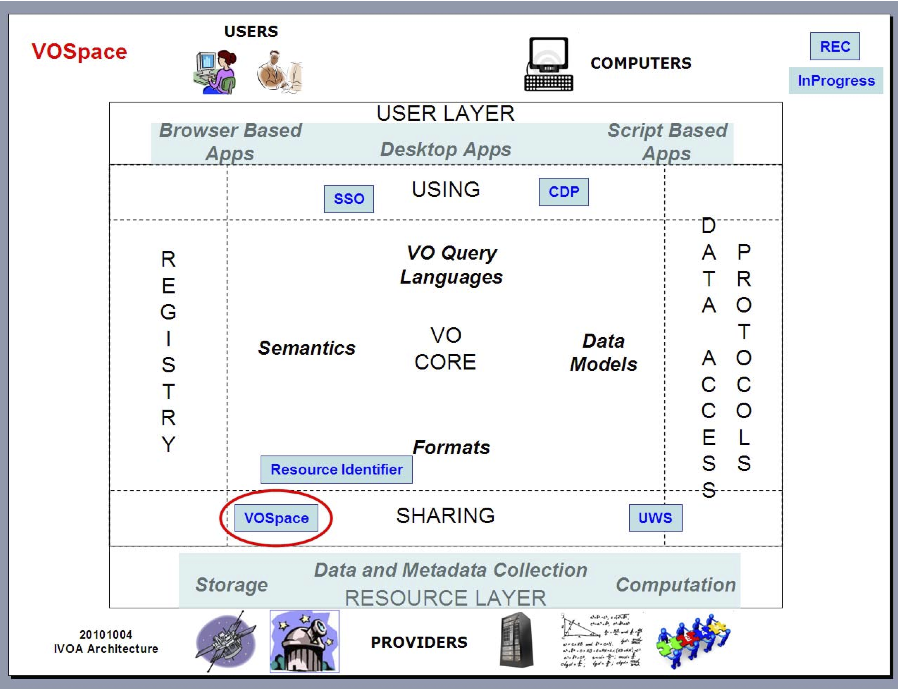
\includegraphics[width=0.9\textwidth]{archdiag.png}
\caption{VOSpace in the IVOA Architecture. This provides an interface to distributed storage. It specifies how applications can use networked data stores to persist and exchange data in a standardized fashion.}
\label{fig:archdiag}
\end{figure}

In this architecture, users employ a variety of tools (from the User Layer) to discover and access archives and services of interest (represented in the Resource Layer). VOSpace provides an interface to storage resources containing the results of using these archives and services and also to other storage solutions, e.g., local disks, where users might want to transfer these results for further work. Items in these resources are referenced by a VOSpace identifier which is related to the standard IVOA Resource Identifier (see section 2). This version of VOSpace employs the UWS design pattern [UWS] to manage data transfers (see section 3.6) and searches (see section 3.7). VOSpace instances may also employ the IVOA Single-Sign-On standard [SSO] for authentication purposes (see section 4) and IVOA Credential Delegation Protocol [CDP] to delegate data transfers.

\subsection{Document roadmap}
The rest of this document is structured as follows:

In Section 2 (TODO: link these section references), we specify the URI syntax for identifying data objects (nodes) in VOSpace.

In Section 3, we present the data model that underpins the VOSpace architecture. This consists of a number of data structures, which have XML representations that are used across the wire in message exchanges with a VOSpace service. These structures represent:

the data objects themselves (nodes)
metadata that can be associated with a data object (properties)
third-party interfaces to the data (capabilities)
the data format used when transferring data objects across the wire (views)
the transport protocol employed in a data transfer (protocols)
the data transfer itself (transfers)
searches of data objects (searches)
We also describe the REST bindings between these representations and their URIs (HTTP identifiers).

In Section 4, we outline how security and access control policies are currently handled in VOSpace.

In Section 5, we detail the operations that the VOSpace interface supports. These handle access to service-level metadata, the creation and manipulation of nodes within the VOSpace, access to node metadata (properties) and data transfer to and from the VOSpace.

In Appendix A, we formally define the VOSpace interface with a machine readable description of its requests and responses and in Appendix B, we present a compliance matrix listing the mandatory behaviour required of a valid VOSpace 2.1 service.

\section{VOSpace identifiers}
The identifier for a node in VOSpace SHALL be a URI with the scheme vos.

Such a URI SHALL have the following parts with the meanings and encoding rules defined in RFC2396 [TODO].

\begin{itemize}
  \item scheme
  \item naming authority
  \item path
  \item (optional) query
  \item (optional) fragment identifier (with the expected semantics [TODO])
\end{itemize}

The naming authority for a VOSpace node SHALL be the VOSpace service through which the node was created. The authority part of the URI SHALL be constructed from the IVO registry identifier [IVORN] for that service by deleting the ivo:// prefix and changing all forward-slash characters('/') in the resource key to exclamation marks ('!') or tildes ('~'). Note that a service SHALL be consistent in its use of separator characters ('!' or '~') when referring to its own data but SHALL accept either as valid in URIs in service requests. For the rest of the document, we shall use '!' as the default character.

This is an example of a possible VOSpace identifier.

\begin{verbatim}
vos://nvo.caltech!vospace/myresults/siap-out-1.vot
\end{verbatim}

The URI scheme is \emph{vos}

Using a separate URI scheme for VOSpace identifiers enables clients to distinguish between IVO registry identifiers and VOSpace identifiers.

\begin{itemize}
    \item nvo.caltech!vospace
\end{itemize}

is the authority part of the URI, corresponding to the IVO registry identifier

\begin{itemize}
    \item ivo://nvo.caltech/vospace
\end{itemize}

This is the IVO registry identifier of the VOSpace service that contains the node.

\begin{itemize}
    \item /siap-out-1.vot is the URI path
\end{itemize}

Slashes in the URI path imply a hierarchical arrangement of data: the data object identified by vos://nvo.caltech!vospace/myresults/siap-out-1.vot is within the container identified by vos://nvo.caltech!vospace/myresults.

Literal space characters are also not allowed in URIs.

All ancestors in the hierarchy SHALL be resolvable as containers (ContainerNodes), all the way up to the root node of the space (this precludes any system of implied hierarchy in the naming scheme for nodes with ancestors that are just logical entities and cannot be reified, e.g. the Amazon S3 system).

A VOSpace identifier is globally unique, and identifies one specific node in a specific VOSpace service.

The standardID for this specification SHALL be: ivo://ivoa.net/std/VOSpace/v2.1.

\subsection{Identifier resolution}
A VOSpace identifier can be resolved to a HTTP endpoint for accessing representations of the node associated with it. A client SHOULD use the following procedure to resolve access to a VOSpace node from a VOSpace identifier:

\begin{itemize}
    \item Resolve HTTP service endpoint of VOSpace service with registry
    \item Append "nodes/" and the path following the naming authority part of the VOSpace identifier to the service endpoint
\end{itemize}

Given the example identifier

\begin{verbatim}
    vos://org.astrogrid.cam!vospace/container-6/siap-out-1.vot?foo=bar
\end{verbatim}

processing the URI to resolve the VOSpace service would involve :

\begin{enumerate}
    \item Extract the IVO registry identifier of the VOSpace service by prepending an ivo scheme to the naming authority part:
        \begin{verbatim}
            ivo://org.astrogrid.cam/vospace
        \end{verbatim}
    \item Resolve the IVO identifier in a registry and retrieve the access URL of the service endpoint:
        \begin{verbatim}
            http://some.uni.ac.uk/vospace
        \end{verbatim}
    \item Append "nodes/" and the path part of the VOSpace identifier:
        \begin{verbatim}
            http://some.uni.ac.uk/vospace/nodes/container-6/siap-out-1.vot?foo=bar
        \end{verbatim}
\end{enumerate}

Note that any fragment identifier in the identifier SHOULD be removed when resolving the identifier to a HTTP endpoint, consistent with the implied semantics of URI fragments [TODO].

\section{VOSpace data model}

\subsection{Nodes and node types}

We refer to the arrangement of data accessible through one particular VOSpace service as "a VOSpace".

Each data object within a VOSpace SHALL be represented as a node that is identified by a URI.

There are different types of nodes and the type of a VOSpace node determines how the VOSpace service stores and interprets the node data.

The types are arranged in a hierarchy (see Figure ~\ref{fig:nodehierarchy}), with more detailed types inheriting the structure of more generic types.

\begin{figure}
\centering
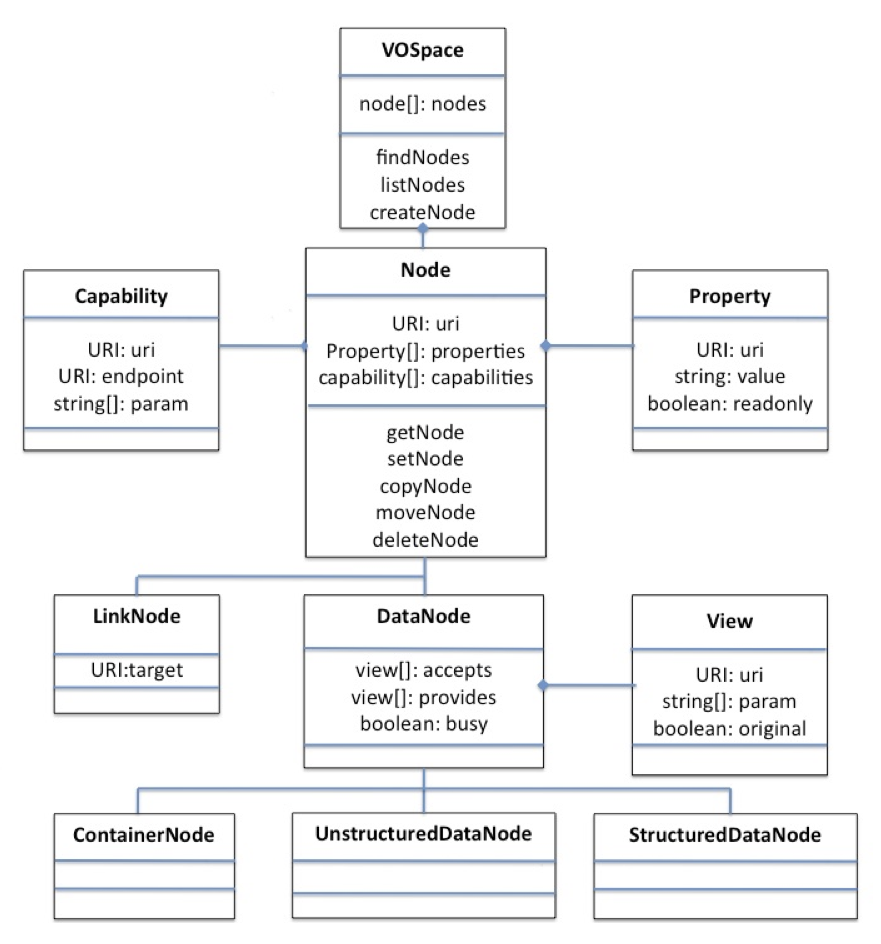
\includegraphics[width=0.9\textwidth]{vospace-node-hierarchy.png}
\caption{Node hierarchy - This shows the inheritance structure for the different types of nodes in VOSpace.}
\label{fig:nodehierarchy}
\end{figure}

The following types (and representations) are defined:

\begin{itemize}
    \item Node is the most basic type
    \item ContainerNode describes a data item that can contain other data items
    \item DataNode describes a data item stored in the VOSpace
    \item UnstructuredDataNode describes a data item for which the VOSpace does not understand the data format
    \item StructuredDataNode describes a data item for which the space understands the format and may make transformations that preserve the meaning of the data.
    \item LinkNode describes a node that points to another node.
\end{itemize}

When data is stored and retrieved from an \emph{UnstructuredDataNode}, the bit pattern read back SHALL be identical to that written.

When data is stored and retrieved from a \emph{StructuredDataNode}, the bit pattern returned MAY be different to the original. For example, storing tabular data from a VOTable file will preserve the tabular data, but any comments in the original XML file may be lost.

A Node representation SHALL have the following elements:

\begin{itemize}
    \item \emph{uri}: the vos:// identifier for the node, URI-encoded according to RFC2396 [TODO]
    \item \emph{properties}: a set of metadata properties for the node
    \item \emph{capabilities}: a third-party interface to a data object
\end{itemize}

In addition, a \emph{DataNode} representation SHALL have the following elements:

\begin{itemize}
    \item \emph{accepts}: a list of the views (data formats) that the node can accept
    \item \emph{provides}: a list of the views (data formats) that the node can provide
    \item \emph{busy}: a boolean flag to indicate that the data associated with the node cannot be accessed
\end{itemize}

The \emph{busy} flag is used to indicate that an internal operation is in progress, and the node data is not available.

A \emph{ContainerNode} representation SHALL have the following elements, in addition to those it inherits from the \emph{Node} representation:

\begin{itemize}
    \item \emph{nodes}: a list of the direct children, if applicable, that the container has. Each child is represented as a node subelement containing its vos:// identifier, URI-encoded according to RFC2396 [TODO]
\end{itemize}

A \emph{LinkNode} representation SHALL have the following elements, in addition to those it inherits from the Node representation:

\begin{itemize}
    \item \emph{target}: the target URI, URI-encoded according to RFC2396 [TODO]
\end{itemize}

The link target can be a URI that points to any type of resource, including other VOSpace Nodes (within the same VOSpace service or in another service), or external resources outside VOSpace altogether.

The properties of a \emph{LinkNode} do not propagate to the target of the \emph{LinkNode}, i.e., a property attached to a LinkNode does not also get attached to the target node. One use case is to enable third-party annotations to be associated with a resource but without the resource itself getting cluttered with unnecessary metadata. In this case, the client creates a \emph{LinkNode} pointing to the resource in question and then adds the annotations as properties of the \emph{LinkNode}.

Both the \emph{ContainerNode} and the \emph{LinkNode} SHALL have no data bytes associated with them.

The set of node types defined by this standard is closed; new types may be introduced only via new versions of the standard.

To comply with the standard, a client or service SHALL be able to parse XML representations of all the node types defined in the current specification.

Note: This does not require all services to support all of the Node types, just that it can process an XML request containing any of the types. If the service receives a request for a type that it does not support, the service SHOULD return a \emph{TypeNotSupported} fault. The service SHALL NOT throw an XML parser error if it receives a request for a type that it does not support.









\appendix
\section{Changes from Previous Versions}

No previous versions yet.  
% these would be subsections "Changes from v. WD-..."
% Use itemize environments.


\bibliography{ivoatex/ivoabib}


\end{document}
